\section{Stregsensor}
På banen til konkurrencen er der en hvid streg, som markerer start. Det ønskes at kunne detektere denne streg, for at vide hvornår bilen har kørt en omgang.\\
Til at dektektere startlinjen, som er hvid, skal den valgte sensor detektere forskellen mellem hvid og sort på banen.\\
 \\
Til det pågældende formål er en reflektiv optisk sensor blevet undersøgt og valgt. Den reflektive optiske sensor har fordelen at den er lille og fylder lidt.\\

\subsection{CNY70}
\begin{wrapfigure}{r}{0.5\textwidth}
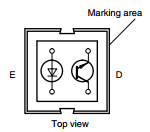
\includegraphics[scale=0.7]{./Graphics/CNY70-Diode}
\caption{Billede af dioden og transisteren i CNY70}
\label{CNY70}
\end{wrapfigure}
Den reflektive optiske sensor som er valgt, hedder CNY70. Sensoren fylder $7x7x6$ mm og er placeret $0.2$ mm fra banen. \\
CNY70'eren er fastmonteret på undervognene af bilen, som vender ned mod banen.\\

Sensoren består af en diode og en fototransistor, som vist i figur \ref{CNY70}, da både diode og fototransistor vender ned mod banen, fungerer den ved at lyset fra dioden reflekteres i banen, hvor fototransistoren opfanger det reflekterede lys. Fototransistoren åbner alt efter hvor meget lys, der bliver reflekteret. \\

\begin{figure}[h!]
\centering
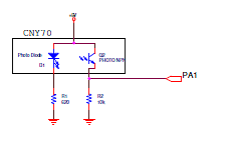
\includegraphics[scale=0.6]{./Graphics/Stregsensor_kredslob}
\caption{Det elektroniske kredsløb over stregsensoren}
\label{Stregsensor}
\end{figure}

Mørke farver absorberer meget af lyset mens lyse farver reflekterer dem. \\
Stregsensoren i figur \ref{Stregsensor} er forsynet med 5V, men kun når diodens stråler reflekteres åbner transistoren, og udgangsspændingen på output-benet bliver højt.\\
Programmet til stregsensoren tjekker først på rising edge\footnote{Se ordliste i afsnit \ref{ordliste}} og registrerer dette, så tjekker den for falling edge\footnote{Se ordliste i afsnit \ref{ordliste}} og registrerer dette, microcontrolleren har nu dektekteret hele målstregen. \\

